\chapter{Resultados e Discussão}\label{cap:resultados}

% \section{Desafio em trajeto especifíco fácil}

% O primeiro e único treino foi executado como agente percorrendo somente um percurso em linha reta, conforme a imagem abaixo.

% \begin{figure}[h]
%     \centering
%     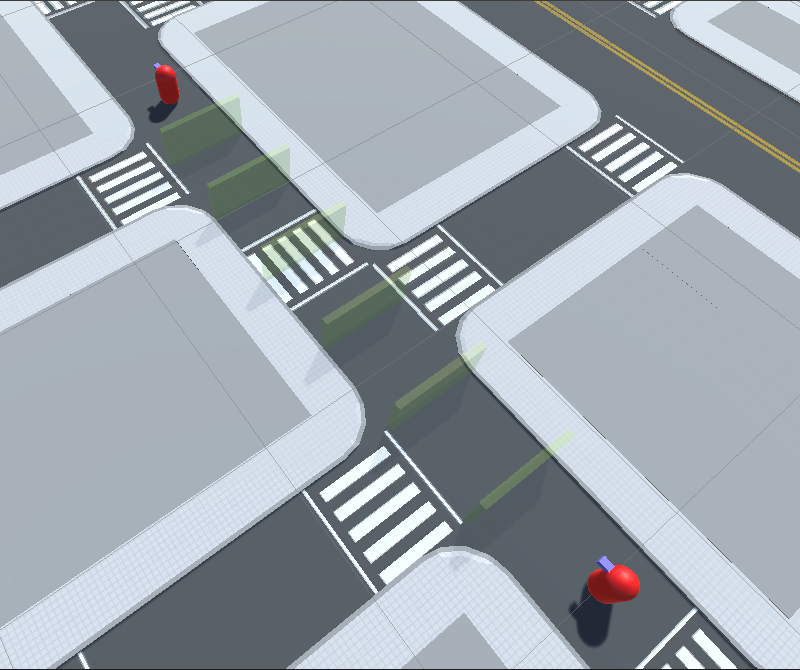
\includegraphics[scale=0.25]{figs/rotas/path_14.png}
%      \caption{O percurso executado no primeiro treino. A cápsula vermelha no canto inferior direito indica a posição inicial do veículo e a na parte superior esquerdo indica o destino.}
%      \label{fig:rota-1}
% \end{figure}
 
% \begin{figure}[h]
%     \centering
%     \includegraphics[scale=0.35]{figs/treinos/treino-1/política.png}
%      \caption{Estatísticas referentes a política. O primeiro gráfico é a entropia, decaindo como é esperado. O terceiro gráfico é o Extrinsic Value estimate, sobe e estabiliza, conforme esperado}
%      \label{fig:treino-1-politica}
% \end{figure}

% \begin{figure}[h]
%     \centering
%     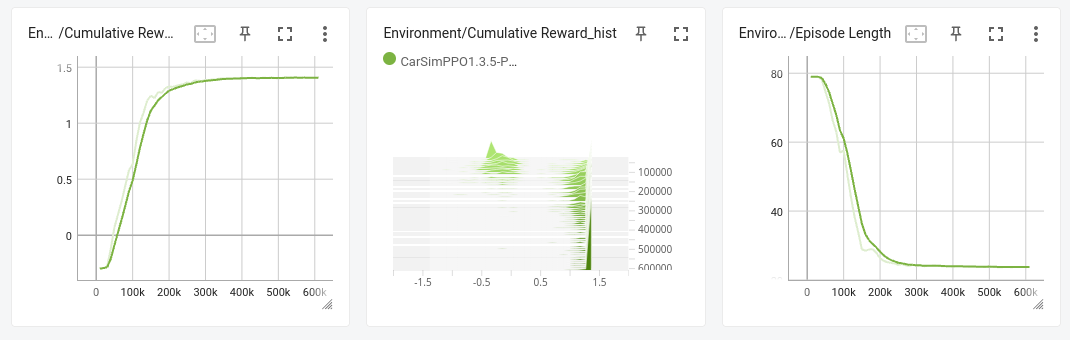
\includegraphics[scale=0.35]{figs/treinos/treino-1/ambiente.png}
%      \caption{Estatísticas do ambiente. O primeiro gráfico é o acumulado de recompensa, o segundo é um histograma das distribuições de recompens. O terceiro é a duração do episódio.}
%      \label{fig:treino-1-ambiente}
% \end{figure}

% \subsection*{Análise}
% O treino foi bem sucedido, o agente soube conduzir bem o veículo. Vendo o gráfico 1 da figura 9, pode-se notar o crescimento exponencial da recompensa e então sua estabilização quando atinge o máximo da recompensa que é possível receber. Também percebe-se que na mesma velocidade mas desta vez em sentido descendente a duração média do episódio, rapidamente cai pois o agente já dominou o trajeto. Isso é o suficiente para este trajeto, podemos treinar o agente em um novo desafio especifíco mas com um trajeto mais complexo.


\section{Desafio em trajeto específico dificuldade fácil}
Aqui o treino foi feito em dois trajetos (identificados por Path(8) e Path(0) no projeto), ambos exigem que o agente faça uma conversão do veículo.

\begin{figure}[h]
    \centering
    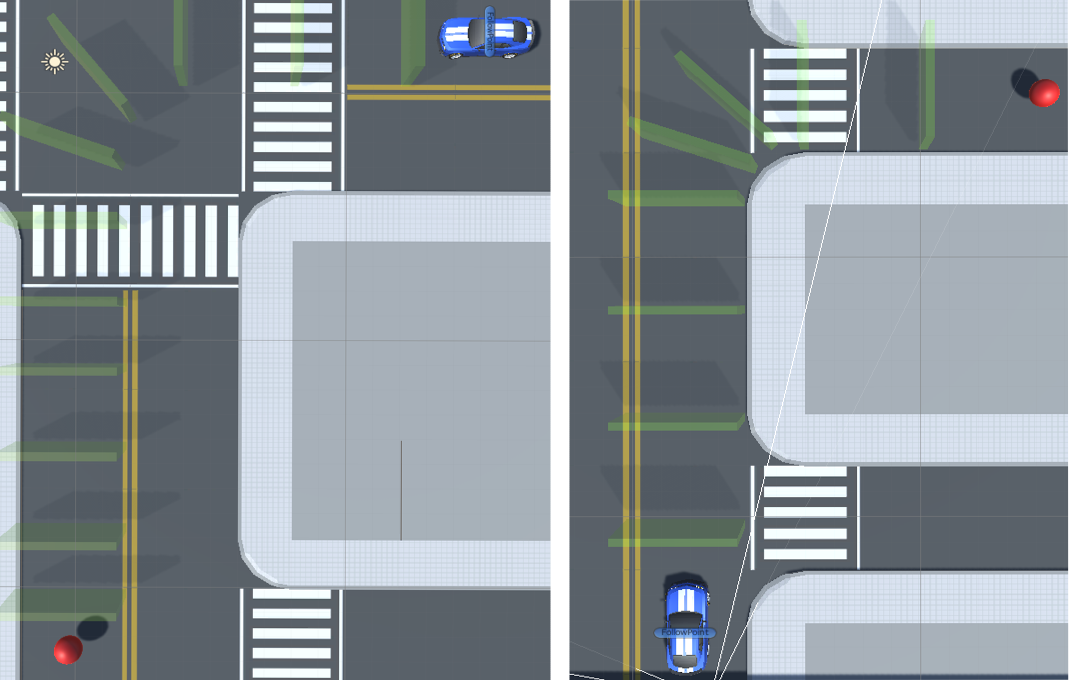
\includegraphics{figs/treinos/desafio-mediano/paths_0-8.png}
    \caption{Trajetos deste desafio, à esquerda o Path(0) e à direita o Path(8).}
\end{figure}

\begin{figure}[h]
    \centering
    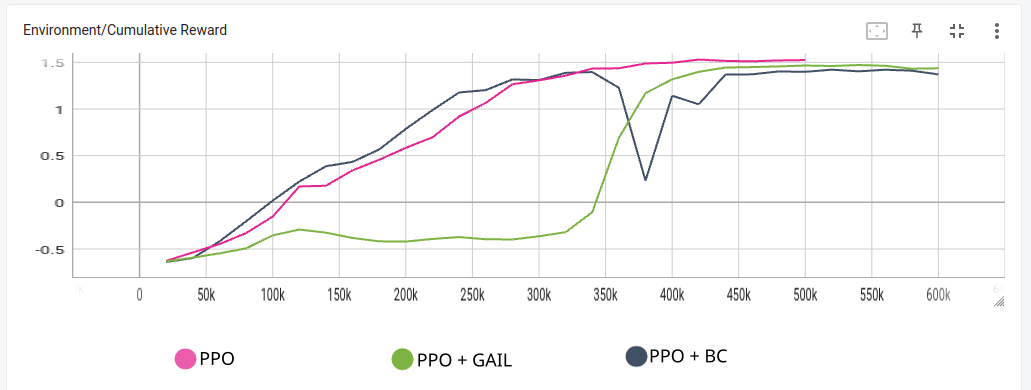
\includegraphics[scale=0.42]{figs/treinos/desafio-mediano/path0/recompensa-ppo-bc-gail-path0.png}
    \caption{Recompensa cumulativa mediana por steps durante o treino do agente no Path(0).}
\end{figure}

\begin{figure}[h]
    \centering
    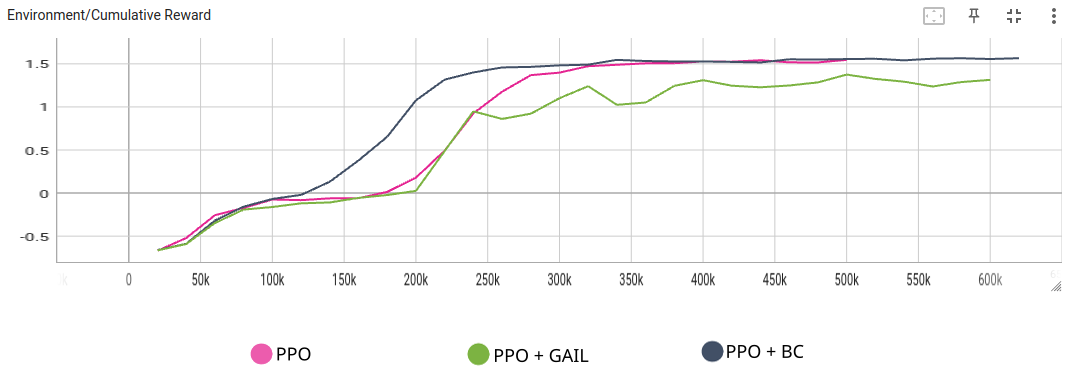
\includegraphics[scale=0.42]{figs/treinos/desafio-mediano/path8/recompensa-ppo-bc-gail-path8.png}
    \caption{Recompensa cumulativa mediana por steps durante o treino do agente no Path(8).}
\end{figure}

O treinamento não encontrou problemas para convergir neste desafio em qualquer dos três algoritmos. PPO foi o que obteve a melhor mediana final no \textit{Path(0)} mesmo dispondo de menos \textit{steps} para treinar. Embora tenham convergido, GAIL e BC se mostrando instáveis, o primeiro demorou muito para mostrar alguma melhora no agente enquanto o último apresentou uma anomalia no Path(0) após 350 mil \textit{steps} voltando a se estabilizar após 450 mil passos. Quanto ao \textit{Path(8)}, o treino utilizando-se de BC convergiu mais rápido e também obteve a maior mediana, enquanto que GAIL foi o mais instável, não convergindo.

\begin{table}[htpb]
    \centering
    \caption{Consolidado de resultados por rota e algoritmo, contém a mediana final da recompensa no treino, o desempenho testes é quantas rotas completou de quantas tentativas e média de recompensas nos testes.}
    \label{resultado-tabela-desafio-1}
    \begin{tabular}{|l|c|c|c|c|c|c|r|}
         \hline
         \small{Rota} & \small{Algoritmo}   & \small{Mediana final rec. treino}  & \small{Desempenho testes}    & \small{Média rec. testes} \\ \hline
            Path(0)   &      PPO            &   1.524                            &    10/10                     &      1                    \\ \hline
            Path(0)   &      GAIL           &   1.436                            &    10/10                     &      1                    \\ \hline
            Path(0)   &      BC             &   1.371                            &    10/10                     &      1                    \\ \hline
            Path(8)   &      PPO            &   1.546                            &    10/10                     &      1                    \\ \hline
            Path(8)   &      GAIL           &   1.314                            &    6/10                      &      0.585                \\ \hline
            Path(8)   &      BC             &   1.565                            &    10/10                     &      1                    \\ \hline
    \end{tabular}
\end{table}


Nos testes, com exceção do algoritmo GAIL no \textit{Path(8)}, foram quase sem qualquer falha. O  cérebro treinado com o algoritmo BC subiu na calçada uma vez em cada teste, mas a punição por uma ocorrência não é suficiente pra afetar a média.

\section{Desafio em trajeto específico difícil}
Para este desafio foi testado em três rotas diferentes: \textit{Path(3), Path(5) e Path(6)}. A primeira é a mais complexa contém três curvas alternadas, enquanto \textit{Path(5)} requer que o carro faça duas conversões a direita e o último trajeto possui duas curvas alternadas. 

Neste desafio ficou claro que o agente teve dificuldade em convergir nos algoritmos BC e GAIL no Path(3), com BC tendo um crescimento constante seguido de uma queda gradual de desempenho até atingir o patamar mais baixo dos três, enquanto GAIL ficou estagnado em um mínimo local assim como fez no Path(5). No Path(6) todos convergiram, com PPO com uma mediana consideravelmente maior.

\begin{figure}[h]
    \centering
    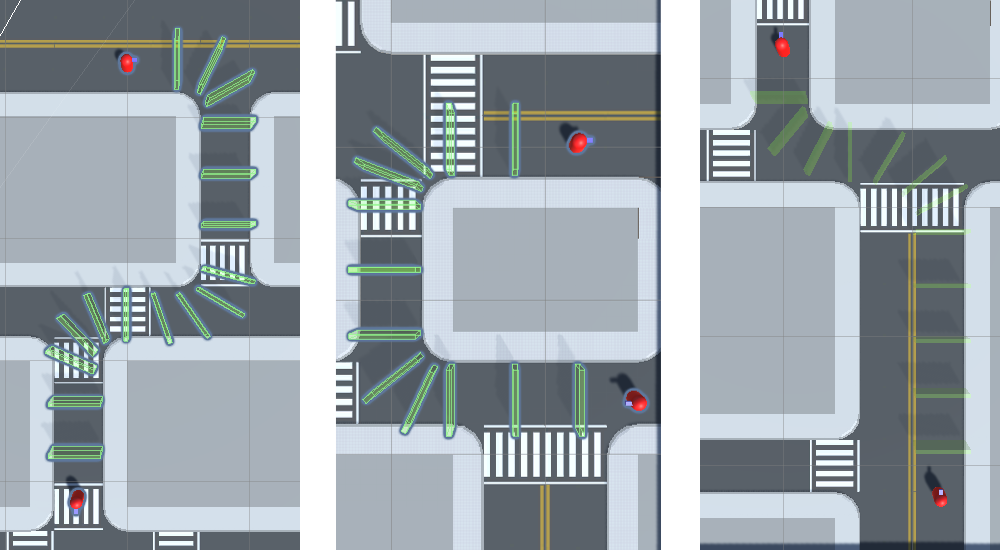
\includegraphics{figs/treinos/desafio-dificil/rotas.png}
    \caption{As três rotas difíceis envolve mais de uma curva, a esquerda o path(3) que possui três curvas sendo o mais complexo dos trajetos. Os outros dois são o path(5) e path(6) que possuem 2 curvas cada.}
\end{figure}

\begin{figure}[h]
    \centering
    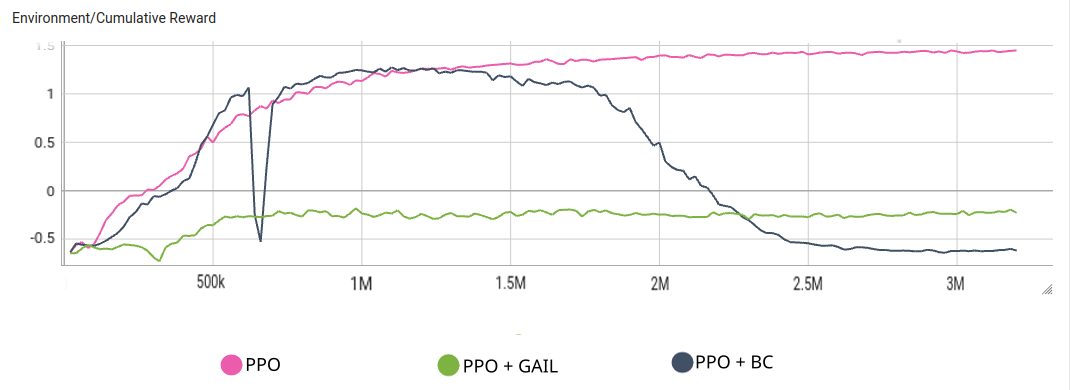
\includegraphics[scale=0.35]{figs/treinos/desafio-dificil/path-3_recompensas-algos.png}
    \caption{Recompensa cumulativa mediana por steps durante o treino do agente no Path(3).}
\end{figure}

\begin{figure}[h]
    \centering
    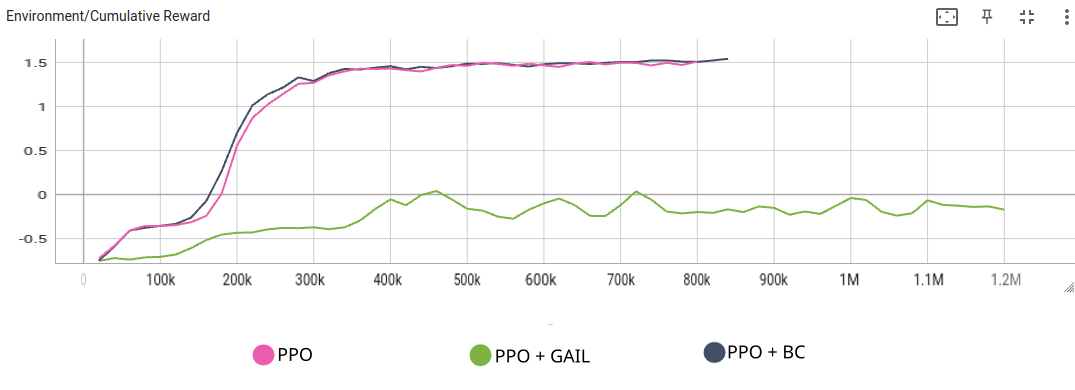
\includegraphics[scale=0.35]{figs/treinos/desafio-dificil/path-5_recompensas-algos.png}
    \caption{Recompensa cumulativa mediana por steps durante o treino do agente no Path(5).}
\end{figure}

\begin{figure}[h]
    \centering
    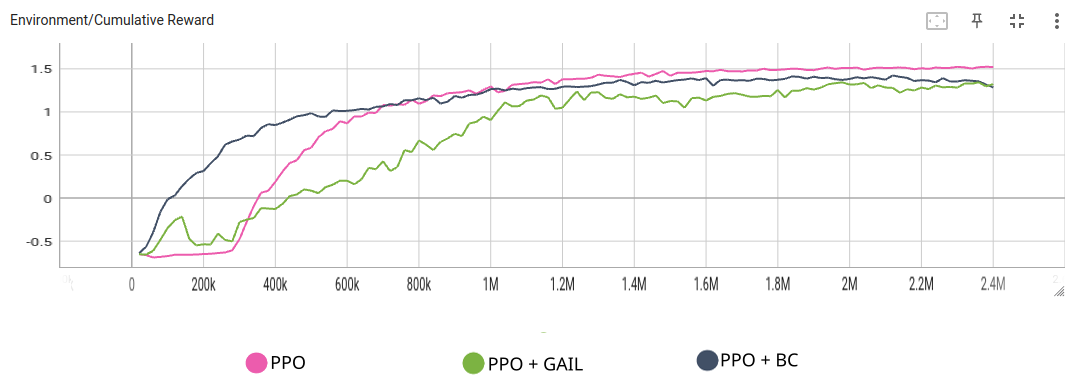
\includegraphics[scale=0.35]{figs/treinos/desafio-dificil/path-6_recompensas-algos.png}
    \caption{Recompensa cumulativa mediana por steps durante o treino do agente no Path(6).}
\end{figure}

\begin{table}[htpb]
    \centering
    \caption{Consolidado de resultados por rota e algoritmo do segundo desafio.}
    \label{resultado-tabela-desafio-2}
    \begin{tabular}{|l|c|c|c|c|c|c|r|}
         \hline
         \small{Rota} & \small{Algoritmo}   & \small{Mediana final rec. treino}  & \small{Desempenho testes}    & \small{Média rec. testes} \\ \hline
            Path(3)   &      PPO            &   1,449                            &    10/10                     &      0,97                 \\ \hline
            Path(3)   &      GAIL           &   -0,229                           &    0/10                      &      -0,261               \\ \hline
            Path(3)   &      BC             &   -0,618                           &    0/10                      &      -0.693               \\ \hline
            Path(5)   &      PPO            &   1,509                            &    10/10                     &      0,98                 \\ \hline
            Path(5)   &      GAIL           &   -0,171                           &    0/10                      &      -0,252               \\ \hline
            Path(5)   &      BC             &   1,505                            &    10/10                     &      1                    \\ \hline
            Path(6)   &      PPO            &   1,522                            &    10/10                     &      0,993                \\ \hline
            Path(6)   &      GAIL           &   1,323                            &    10/10                     &      0,99                 \\ \hline
            Path(6)   &      BC             &   1,284                            &    5/10                      &      0,42                 \\ \hline
    \end{tabular}
\end{table}

Todos desempenharam de acordo com o treino durante os testes com exceção do BC no Path(6) concluiu apenas metade das rotas. Durante o teste do Path(6) foi observado uma diferença interessante entre o agente treinado com PPO que usa apenas RL e o GAIL que utiliza-se de IL: o primeiro tendia a abusar de uma falha de detecção de colisão do veículo com a calçada poupando assim um pouco de tempo (e de punição por step) em vez de seguir na via. Isso ocorre porque da forma que o agente passa sobre a calçada o modelo raramente detecta uma colisão ali, com o agente treinado em GAIL isto não ocorre, já que o mesmo tenta imitar o comportamento na demonstração feita por um humano que seguiu na via normalmente.

\section{Desafio em todos os trajetos}
Neste desafio houve uma discrepância muito grande entre GAIL e os outros dois, este último não teve um treino estável mesmo após diversos ajustes nos hiperparâmetros e isto refletiu nos testes onde obteve uma recompensa média negativa. Nas tabelas \ref{resultado-tabela-geral-ppo} e \ref{resultado-tabela-geral-bc} pode-se ver que ambos tiveram mais dificuldades no \textit{Path(10)} que possui duas curvas pra esquerda. Interessante ressaltar que BC nestes testes conseguiu concluir o Path(3) em todas as tentativas em contraste com o desafio anterior onde falhou em todas as dez tentativas, o que nos leva a crer que treinar em outros trajetos ajude o agente a cumprir um trajeto específico em vez de treinar somente em um único trajeto, pelo menos utilizando-se de Aprendizado por Imitação.

\begin{figure}[h]
    \centering
    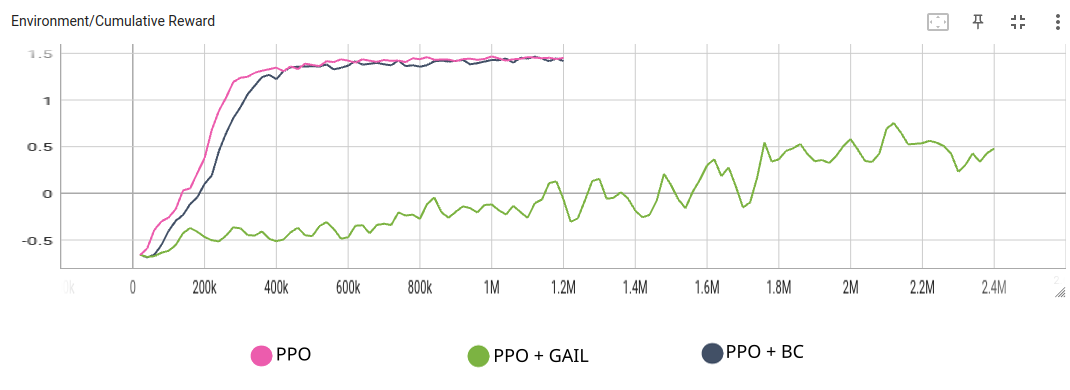
\includegraphics[scale=0.35]{figs/treinos/desafio-geral/recompensa-ppo-gail-bc.png}
    \caption{Recompensa cumulativa mediana por steps durante o treino do agente em todos os trajetos.}
\end{figure}

\begin{table}[htpb]
    \centering
    \caption{Detalhamento do desempenho no teste do desafio geral de PPO, inclui todas tentativas e suas recompensas e a recompensa média por rota.}
    \label{resultado-tabela-geral-ppo}
    \begin{tabular}{|l|c|c|c|c|c|c|r|}
         \hline
         \multirow{2}{*}{Rota} & \multicolumn{2}{c|}{Tentativa 1}  & \multicolumn{2}{c|}{Tentativa 2} & \multicolumn{2}{c|}{Tentativa 3} & \multirow{2}{*}{Rec. média} \\ \cline{2-7}
                               & \small{Concluiu?}  & \small{Rec.} & \small{Concluiu?} &\small{Rec.} & \small{Concluiu?} &\small{Rec.} &                               \\ \hline
            Path(0)   &      sim        &   1             &    sim          &      1        &    sim          &      1        &      1                 \\ \hline
            Path(1)   &      sim        &   1             &    sim          &      1        &    sim          &      1        &      1                 \\ \hline
            Path(2)   &      sim        &   1             &    sim          &      1        &    sim          &      1        &      1                 \\ \hline
            Path(3)   &      não        &   -0,18         &    sim          &      0,85     &    sim          &      1        &      0,56              \\ \hline
            Path(4)   &      sim        &   1             &    sim          &      1        &    sim          &      1        &      1                 \\ \hline
            Path(5)   &      sim        &   1             &    sim          &      0,8      &    sim          &      1        &      0,93              \\ \hline
            Path(6)   &      sim        &   1             &    não          &      -0,31    &    sim          &      1        &      0,56              \\ \hline
            Path(7)   &      sim        &   0,85          &    sim          &      1        &    sim          &      0,9      &      0,91              \\ \hline
            Path(8)   &      sim        &   1             &    sim          &      0,9      &    sim          &      1        &      0,96              \\ \hline
            Path(9)   &      sim        &   1             &    sim          &      0,95     &    sim          &      1        &      0,98              \\ \hline
            Path(10)  &      não        &   0,12          &    não          &      0,02     &    sim          &      1        &      0,38              \\ \hline
            Path(11)  &      sim        &   1             &    sim          &      1        &    sim          &      1        &      1                 \\ \hline
            Path(12)  &      sim        &   1             &    sim          &      1        &    sim          &      1        &      1                 \\ \hline
            Path(13)  &      sim        &   1             &    sim          &      1        &    sim          &      1        &      1                 \\ \hline
            Path(14)  &      sim        &   1             &    sim          &      1        &    sim          &      1        &      1                 \\ \hline
            Path(15)  &      sim        &   1             &    sim          &      1        &    sim          &      1        &      1                 \\ \hline
            Path(16)  &      sim        &   1             &    sim          &      1        &    sim          &      1        &      1                 \\ \hline
    \end{tabular}
\end{table}

\begin{table}[htpb]
    \centering
    \caption{Detalhamento do desempenho no teste do desafio geral de GAIL.}
    \label{resultado-tabela-geral-gail}
    \begin{tabular}{|l|c|c|c|c|c|c|r|}
         \hline
         \multirow{2}{*}{Rota} & \multicolumn{2}{c|}{Tentativa 1}  & \multicolumn{2}{c|}{Tentativa 2} & \multicolumn{2}{c|}{Tentativa 3} & \multirow{2}{*}{Rec. média} \\ \cline{2-7}
                               & \small{Concluiu?}  & \small{Rec.} & \small{Concluiu?} &\small{Rec.} & \small{Concluiu?} &\small{Rec.} &                               \\ \hline
            Path(0)            &      sim          &   1          &    não            &      -0,677 &    sim            &      -0,402 &      -0,026                    \\ \hline
            Path(1)            &      não          &   0,231      &    não            &      -0,01  &    não            &      -0,253 &      -0,011                    \\ \hline
            Path(2)            &      não          &   -0,375     &    não            &      -0,153 &    não            &      -0,551 &      -0,36                     \\ \hline
            Path(3)            &      não          &   -0.412     &    não            &      0,002  &    não            &      -0,588 &      -0,333                    \\ \hline
            Path(4)            &      não          &   -0,086     &    sim            &      1      &    não            &      -0,504 &      0,137                     \\ \hline
            Path(5)            &      não          &   -0,278     &    não            &      0,132  &    não            &      -0,515 &      -0,22                     \\ \hline
            Path(6)            &      sim          &   1          &    sim            &      1      &    não            &      0,201  &      0,734                     \\ \hline
            Path(7)            &      não          &   -0,297     &    não            &      -0,22  &    não            &      -0,636 &      -0,384                    \\ \hline
            Path(8)            &      não          &   0,087      &    não            &      -0,087 &    não            &      0,215  &      0,072                     \\ \hline
            Path(9)            &      não          &   -0,084     &    não            &      0,204  &    não            &      -0,104 &      0,006                     \\ \hline
            Path(10)           &      não          &   -0,44      &    não            &      -0,677 &    não            &      -0,586 &      -0,566                    \\ \hline
            Path(11)           &      não          &   0,063      &    não            &      -0,182 &    sim            &      1      &      0,293                     \\ \hline
            Path(12)           &      não          &   0,074      &    não            &      -0,44  &    não            &      -0,655 &      -0,292                    \\ \hline
            Path(13)           &      nào          &   0,191      &    não            &      -0,686 &    não            &      -0,668 &      -0,718                    \\ \hline
            Path(14)           &      não          &   0,098      &    não            &      -0,644 &    não            &      -0,553 &      -0,366                    \\ \hline
            Path(15)           &      não          &   -0,579     &    não            &      -0,397 &    não            &      -0,47  &      -0,604                    \\ \hline
            Path(16)           &      sim          &   1          &    não            &      -0,665 &    não            &      -0,653 &      -0,106                    \\ \hline
    \end{tabular}
\end{table}

\begin{table}[htpb]
    \centering
    \caption{Detalhamento do desempenho no teste do desafio geral de BC.}
    \label{resultado-tabela-geral-bc}
    \begin{tabular}{|l|c|c|c|c|c|c|r|}
         \hline
         \multirow{2}{*}{Rota} & \multicolumn{2}{c|}{Tentativa 1}  & \multicolumn{2}{c|}{Tentativa 2} & \multicolumn{2}{c|}{Tentativa 3} & \multirow{2}{*}{Rec. média} \\ \cline{2-7}
                               & \small{Concluiu?}  & \small{Rec.} & \small{Concluiu?} &\small{Rec.} & \small{Concluiu?} &\small{Rec.} &                               \\ \hline
            Path(0)   &      sim        &   1             &    sim          &      1        &    sim          &      1        &      1                 \\ \hline
            Path(1)   &      sim        &   1             &    sim          &      1        &    sim          &      1        &      1                 \\ \hline
            Path(2)   &      sim        &   1             &    sim          &      1        &    sim          &      1        &      1                 \\ \hline
            Path(3)   &      sim        &   1             &    sim          &      0,9      &    sim          &      1        &      0.967             \\ \hline
            Path(4)   &      sim        &   1             &    sim          &      1        &    sim          &      1        &      1                 \\ \hline
            Path(5)   &      sim        &   1             &    sim          &      1        &    sim          &      1        &      1                 \\ \hline
            Path(6)   &      sim        &   1             &    sim          &      1        &    sim          &      1        &      1                 \\ \hline
            Path(7)   &      sim        &   1             &    sim          &      0,95     &    sim          &      1        &      0,983             \\ \hline
            Path(8)   &      sim        &   1             &    sim          &      0,95     &    sim          &      1        &      0,983             \\ \hline
            Path(9)   &      sim        &   1             &    sim          &      1        &    sim          &      1        &      1                 \\ \hline
            Path(10)  &      não        &   0,224         &    não          &      0,158    &    não          &      0,221    &      0,201             \\ \hline
            Path(11)  &      sim        &   1             &    sim          &      1        &    sim          &      1        &      1                 \\ \hline
            Path(12)  &      sim        &   1             &    sim          &      1        &    não          &      -0,41    &      0,53              \\ \hline
            Path(13)  &      sim        &   1             &    sim          &      1        &    sim          &      1        &      1                 \\ \hline
            Path(14)  &      sim        &   1             &    sim          &      1        &    sim          &      1        &      1                 \\ \hline
            Path(15)  &      sim        &   1             &    sim          &      1        &    não          &      0,12     &      0,707             \\ \hline
            Path(16)  &      sim        &   1             &    sim          &      1        &    sim          &      1        &      1                 \\ \hline
    \end{tabular}
\end{table}


\begin{table}[htpb]
    \centering
    \caption{Consolidado de resultados no desafio geral.}
    \label{resultado-tabela-desafio-geral}
    \begin{tabular}{|l|c|c|c|r|}
         \hline
         \small{Rota}           & \small{Algoritmo}   & \small{Mediana final rec. treino}  & \small{Desempenho testes}    & \small{Média rec. testes} \\ \hline
         \multirow{3}{*}{Todas} &      PPO            &   1,451                            &    47/51                     &      0,899                \\ \cline{2-5}
                                &      GAIL           &   0,479                            &    7/51                      &      -0,161               \\ \cline{2-5}
                                &      BC             &   1,416                            &    46/51                     &      0,904                \\ \hline
    \end{tabular}
\end{table}